%\documentclass[12pt,a4paper,twoside]{book} 
\usepackage[spanish]{babel} % de pedro
\usepackage{graphics,graphicx,epsfig,color,float,afterpage,fancyheadings,subfigure,moreverb,alltt} % de pedro
\usepackage[latin1]{inputenc} % tildes de pedro

\usepackage{algorithm}
\usepackage{algorithmic}

\usepackage{rotating}
\usepackage{url}

%% Esta letra se convierte mejor a pdf que la normal
\usepackage{ae}

%%% Para las fuentes matemticas
\usepackage{amsfonts}

\usepackage{subfigure}

\usepackage{pstricks} % para los dibujos del da
\usepackage{lscape} % para las pginas en horizontal
\usepackage{portland} % para las pginas en horizontal
\usepackage{supertabular} % para las tablas de ms de una pgina
\usepackage{tabularx} % para las tablas del tipo tabularx
%\usepackage{glossary}
%\documentclass[a4paper,spanish,12pt]{book} % esto es de gustavo
%\usepackage{amsmath,amsfonts}   % underset mathbb
%\usepackage{authordate1-4}      % bib style
%\usepackage{epsfig}     % eps
\usepackage{epic}           % graficos
%\usepackage{eepic}           % graficos
\usepackage{curvesls}           % curvas
\usepackage{amssymb}
%\usepackage{fancyheadings}  % encabezados
%\usepackage{hhline}             % hhline
%\usepackage[latin1]{inputenc}   % tildes
%\usepackage{makeidx}        % ndices
%\usepackage{setspace}           % interlinea
%\usepackage[spanish]{babel} % espaol

%%%%%%%%%%%%%%%%%%%%%%%%%%%%%%%%%%%%%%%%%%%%%%%%%%%%%%%%%%%%%%%%%%%%%%%%%%%%%%%

\author{juanlu}
\title{Tesis de Juan Lus Jimnez Laredo}




\newcommand{\fecha}{\footnotesize{[ Impreso: \the\day-\ifcase\month\or
    Ene\or Feb\or Mar\or Abr\or May\or Jun\or Jul\or Ago\or Sep\or
      Oct\or Nov\or Dic\fi-\the\year ]}}

\newcommand{\N}{\mathbb{N}}

%% Para corregir las cabeceras largas
\newcommand{\cabecera}[2]{
\markright{\ref{#1}. \hspace{0.1ex} \MakeUppercase{#2}}}


%\pagestyle{headings}
%\renewcommand{\chaptermark}[1]{\markboth{\fecha \\ \\ #1}{}}
%\renewcommand{\sectionmark}[1]{\markright{#1 \\ \\ \fecha}}
%\addtolength{\headheight}{2.5pt}



%\lhead[\it\thechapter]{\sl\rightmark}
%\rhead[\rm\leftmark]{\it\thesection}
%\rfoot[]{\thepage}
%\cfoot[]{}
%\lfoot[\thepage]{}

%\thispagestyle{plain}

\setcounter{secnumdepth}{3}
\setcounter{tocdepth}{3}

%\renewcommand{\baselinestretch}{1.2}
%\setlength{\parskip}{0.8ex}

\newtheorem{theorem}{\sf Teorema}
\newtheorem{lemma}{\sf Lema}

\newcommand{\rem}[1]{\S\iffalse #1 \fi}
\newcommand{\cur}[1]{ {\it #1\/} }
\newcommand{\crcl}[1]{#1\kern-9pt\raise1pt\hbox{$\bigcirc$}}
\newcommand{\evag}{{\sf EvAg}}
\newcommand{\evagp}{{\sf EvAg.}}
\newcommand{\evags}{{\sf EvAgs}}
\newcommand{\evagsp}{{\sf EvAgs.}}

\newcommand{\prog}[2] {
   \small
   \begin{minipage}[t]{75mm} {\tt #1}  \end{minipage}
   \begin{minipage}[t]{60mm} {#2}      \end{minipage}
   \\
}
\newcommand{\prg}[2] { {\tt #1} & {\sf #2} \\}

\newcommand{\wmfspecial}[4]{
   \begin{figure}[h]
   \centerline{\psfig{figure=#1,height=#2}}
   \caption{#3}   \label{#4}
   \end{figure}
}                   % USO: \wmfspecial{nombre.eps}{altura}{leyenda}{etiqueta}

\def\stackunder#1#2{\mathrel{\mathop{#2}\limits_{#1}}}

\def\marco #1#2#3#4{\centerline{       % USO: \marco{.1}{10}{124mm}
  \vbox{\hrule height #1pt%
  \hbox{\vrule width #1pt\kern #2pt%
  \vbox{\kern #2pt%
  \vbox{\hsize #3\noindent #4}%
  \kern #2pt}%
  \kern #2pt\vrule width #1pt}%
  \hrule height0pt depth #1pt}} }


\newcommand{\symnote}[2]{\symbolnote{#1}{#2}}

\newfont{\bi}{cmbxti10 scaled\magstep1}       % bf + it


%% Ruta de las figuras
\graphicspath{{../figuras/}}


\begin{document}
           % Eliminarlo al compilar el documento maestro, ponerlo para compilarlo separado

%%%%%%%%%%%%%%%%%%%%%%%%%%%%%%%%%%%%%%%%%%%%%%%%%%%%%%%%%%%%%%%%%%%%%%%%%%%%%%%
%%                                                                           %%
%%                             Tesis Doctoral:                               %%
%%                        Juan Luis Jimenez Laredo                           %%
%%                                                                           %%
%%%%%%%%%%%%%%%%%%%%%%%%%%%%%%%%%%%%%%%%%%%%%%%%%%%%%%%%%%%%%%%%%%%%%%%%%%%%%%%


\cabecera{cap:peas}{Parallel and Distributed Evolutionary Algorithms} %Descomentarlo para compilar maestro
\chapter{\textit{Parallel and Distributed Evolutionary Algorithms}}
\label{cap:peas}
\cabecera{cap:peas}{Parallel and Distributed Evolutionary Algorithms} %Descomentarlo para compilar maestro


As saw in chapter \ref{cap:introduccion}, computational efforts in EAs can be high for demanding problems with parallelisation arising as a way of improving the algorithm performance. In that context, a good knowledge of adequate parallel models turns into a key for providing efficient designs.
 
 

%Therefore, a good knowledge on the computer architecture of the underlying platform is key to adopt an adequate model of parallelisation.


%EAs are a set of population-based stochastic search techniques able to solve optimisation problems in reasonable time. However, for very demanding applications and large problem instances the computational efforts (execution times) of EAs can be high. Fortunately, EAs are rather easy to execute in a parallel fashion offering a straightforward way to improve scale-up properties. The nature of EAs is inherently suited to be parallelised at population level in which the main idea is to speedup the execution time of the algorithm by sharing the workload of the individuals among a pool of processors. Therefore, a good knowledge on the computer architecture of the underlying platform is key to adopt an adequate model of parallelisation.

This chapter introduces a general overview on the most extended models of parallel and distributed EAs in Section \ref{sec:pdeas}. Rather than presenting an exhaustive analysis, the aim is to establish a global framework to help understanding the following chapters in the concrete computer architecture area of P2P Computing. This way, Section \ref{sec:structurecomplex} provides some keys on how complex systems, such as P2P, can host distributed EAs by structuring the population with the shape of a complex network. Finally, Section \ref{sec:p2peas} complements the view with the most relevant approaches to P2P EAs in the literature.


As a final consideration, we have adopted the following criterion for the alternate use of the concepts {\em parallel} and {\em distributed}. By {\em parallel} we will refer to the property of an EA to be subdivided in sub-tasks that can be executed with a certain degree of independence. On the other hand, {\em distributed} refers to the parallel quality of several sub-tasks for being executed in a loosely-coupled fashion (e.g. in distributed memory systems in which every processor access its own private memory) \cite{peleg00:distributed,friedman08:distributed}.


% El hecho de que el fichero se llame pea y no dea implica que son tan
% parecidos que posiblemente sea conveniente que definas DEA, y hables
% de la diferencias con los paralelos, por ejemplo - JJ
% Es cierto, ahora hablo de "Parallel and Distributed Evolutionary Algorithms" y especifico las diferencias en este último párrafo - Juanlu







%%%%%%%%%%%%%%%%%%%%%%%%%%%%%%%%%%%%%%%%%%%%%%%%%%%%%%%%%%%%%
\section{Parallel and Distributed Evolutionary Algorithms models}
\label{sec:pdeas}
%%%%%%%%%%%%%%%%%%%%%%%%%%%%%%%%%%%%%%%%%%%%%%%%%%%%%%%%%%%%%


Parallel and Distributed EAs models face two different aspects, the algorithmic and the computational performance. The first is related to the changes that the algorithm structure suffers when deployed on several processors while the latter corresponds to the computational speedup that can be expected. In fact, parallel EAs are studied as a way of preserving genetic diversity while improving the execution time of the algorithm. 

The following sections present different models of parallelisation showing that not all of them fit well with P2P systems due to issues such as decentralisation, massive scalability or fault-tolerance. The parallel models are presented in two main groups according with the classification of Alba and Tomassini in \cite{alba:parallelism}: 

%%%%%%%%%%%%%%%%%%%%%%
\begin{itemize}
\item Global parallel EAs (Section \ref{sec:masterslave}) in which there is a single population that follows the panmictic scheme of reproduction of a sequential EA. In such an approach, parallelism lies in the parallel evaluation of individuals and sometimes the parallel application of the genetic operators.

\item Spatially structured EAs in which the parallelism is present at population level. The purpose is to balance the algorithm workload by spatially structuring the population of individuals among the available processors. Sections \ref{sec:coarsegrained} and \ref{sec:finegrained} present different approaches to spatially structured EAs depending on the parallelisation grain.

\end{itemize}
%%%%%%%%%%%%%%%%%%%%%%


%%%%%%%%%%%%%%%%%%%%%%%%%%%%%%%%%%%%%%%%%%%%%%%%%%%%%%%%%%%%%
\subsection{Global parallel evolutionary algorithms}
\label{sec:masterslave}
%%%%%%%%%%%%%%%%%%%%%%%%%%%%%%%%%%%%%%%%%%%%%%%%%%%%%%%%%%%%%

This approach takes advantage of the parallelism at evaluation level in the case of very demanding \emph{fitness} evaluation functions. Global parallelisation consists in the parallel evaluation of the individuals, usually following the {\em master-slave model} depicted in Figure \ref{fig:masterslave} in which the algorithm runs on the master node and the individuals are sent for evaluation to the slaves. Additionally, the master is responsible for collecting the results and applying the genetic operators. Therefore, scalability is often limited by the master performance and the incoming bandwidth leading to sublinear speedups. For instance, Hauser and M\"anner in \cite{hauser94} report an speedup of 5 using 6 processors. Abramson et al. in \cite{abramson93} hold a linear speedup up to 16 processors in a 128 processor architecture. Finally, Cant\'u-Paz points in \cite{cantu:parallelga} that speedup degrades quickly using such a model as a consequence of the master acting as a bottleneck in distributed memory computers. Therefore, we can conclude that global parallelisation models do not fit with the P2P systems requirements on massive scalability.


      %Which is bad because ... en general, ningún sistema se plantea en
      %un entorno donde se rompan los ordenadores. si vas a ``trabajar''
      %en ese entorno, dilo desde el principio y luego justifica este
      %tipo de cosas... - JJ
      % Often? How often? Siempre
      % cita! Recuerda, esto no es un trabajo en un congreso, debes
      % probar absolutamente todo y no dejar cabos sueltos. Tampoco
      % tienes limite de páginas ni de citas.

%% He añadido tres referencias, a cantú-paz, hauser y abramson justificando la falta de escalabilidad en estos sistemas - Juanlu

\begin{figure}[htbp]
\centering
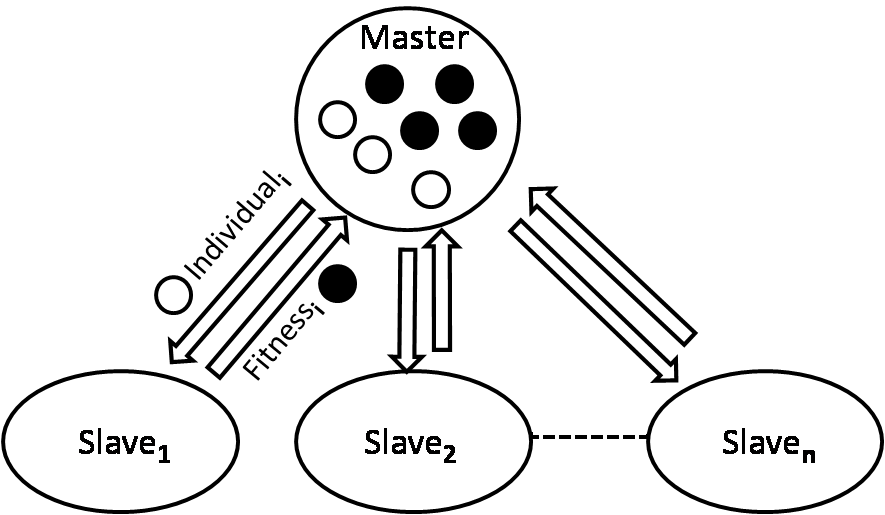
\includegraphics[width=0.5\textwidth]{masterslave}
\caption{Global parallel evolutionary algorithms. Master-Slave model.}
\label{fig:masterslave}
\end{figure}



%%%%%%%%%%%%%%%%%%%%%%%%%%%%%%%%%%%%%%%%%%%%%%%%%%%%%%%%%%%%%
\subsection{Spatially structured coarse-grained approaches}
\label{sec:coarsegrained}
%%%%%%%%%%%%%%%%%%%%%%%%%%%%%%%%%%%%%%%%%%%%%%%%%%%%%%%%%%%%%

One of the most usual and widely studied coarse-grained approaches is the {\em Island model} depicted in Figure \ref{fig:islandmodel}. As described by Cant\'u-Paz in \cite{cantu99:topologies}, the idea behind this model is that the global panmictic population is split in several sub-populations or demes called islands. The communication between islands is defined by a given topology, through which they exchange individuals (migrants) with a certain rate and frequency. The migration follows a selection policy in the source island and a replacement policy in the target one. 

Practitioners generally use a fixed population size $P$ in studies of scalability, a maximum number of islands $N$ and a population size per island of $P/n$ where $n = 1,\dots,N$. That is the case described by Hidalgo and Fern\'andez in \cite{Fernandez:balancing} where the authors show how the algorithmic results are highly sensitive to the calibration of the multiple parameters, and in particular, to the number of islands. Specifically, the best algorithmic result is obtained using a single island, that is, a sequential EA. In addition, the authors conclude that using a small number of individuals per island is usually a bad choice. Such results are in consonance with those of Cant\'u-Paz and Goldberg in \cite{cantu:singlerun} suggesting that for difficult problems (large problem instances with high-order BBs) the best choice is using a single deme with a large population. Therefore, the island model turns into an unsuitable alternative for P2P systems, given that, distributed EAs over P2P systems  have to focus on the efficient load-balance of a population among a large amount of resources in order to tackle large problem instances. 

\begin{figure}[htbp]
\centering
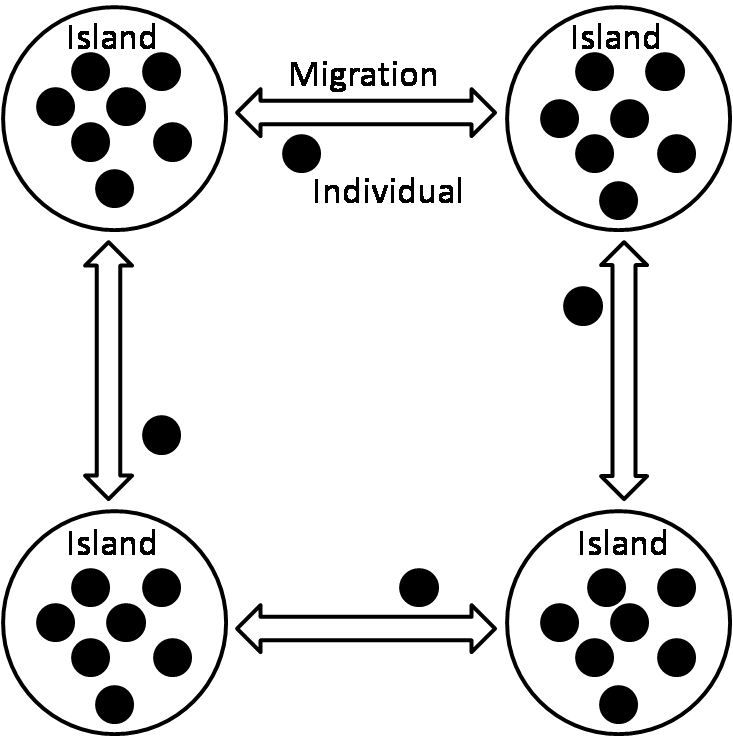
\includegraphics[width=0.5\textwidth]{islands}
\caption{Spatially structured coarse-grained approach. Island model.}
\label{fig:islandmodel}
\end{figure}


%%%%%%%%%%%%%%%%%%%%%%%%%%%%%%%%%%%%%%%%%%%%%%%%%%%%%%%%%%%%%
\subsection{Spatially structured fine-grained approaches}
\label{sec:finegrained}
%%%%%%%%%%%%%%%%%%%%%%%%%%%%%%%%%%%%%%%%%%%%%%%%%%%%%%%%%%%%%


In {\em fine-grained approaches} every individual in the population is placed on its own processor and evolves within a defined neighbourhood. One of the most common fine-grained approaches is the Cellular Evolutionary Algorithm (CEA) \cite{alba:cga}. Individuals in CEAs are usually disposed in n-dimensional grid lattices  as depicted in Figure \ref{fig:finegrained} (a) where the mate choice is restricted to those individuals in the neighbourhood, thus, unlike in panmictic EAs, selection is decentralised. 


Most of the efforts in CEAs have focused on analysing the algorithmic effects of using different neighbourhood policies. For example, Giacobini studies in \cite{giacobini:regular} the impact of regular lattices on the selection pressure and of different graph structures such a toroid in \cite{giacobini:gecco04}. Dorronsoro et al. 
 study in \cite{dagt04} the effect of different grid shapes and asynchrony in CEAs. However, fine-grained approaches are not only subject to regular population structures and there are some interesting results considering complex networks as population structure (see Figure \ref{fig:finegrained} (b)).  Giacobini et al. analyse in \cite{giacobini:gecco05} the influence of random and small-world structured populations on the selection pressure and empirically demonstrate in \cite{giacobini:evocop06} that complex network population structures are competitive against panmictic EAs. Such results show the suitability of the fine-grained approach for decentralised systems as P2P system since they are inherently organised as complex networks.


\begin{figure}[htbp]
\centering
\subfigure[Regular lattice neighbourhood.]{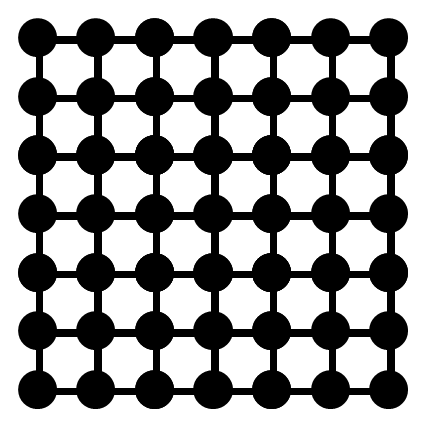
\includegraphics[width=0.4\textwidth]{cea}}
\subfigure[Complex network neighbourhood.]{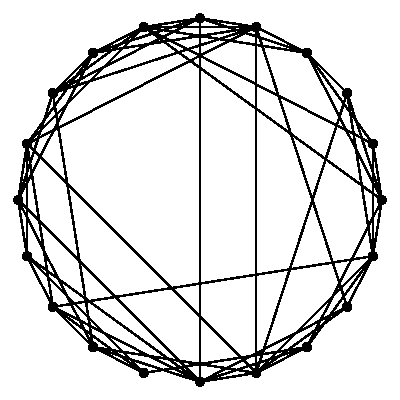
\includegraphics[width=0.4\textwidth]{WS-20-0200}}
\caption{Spatially structured fine-grained approaches.}
\label{fig:finegrained}
\end{figure}



%\begin{figure}[htbp]
%\centering
%\subfigure{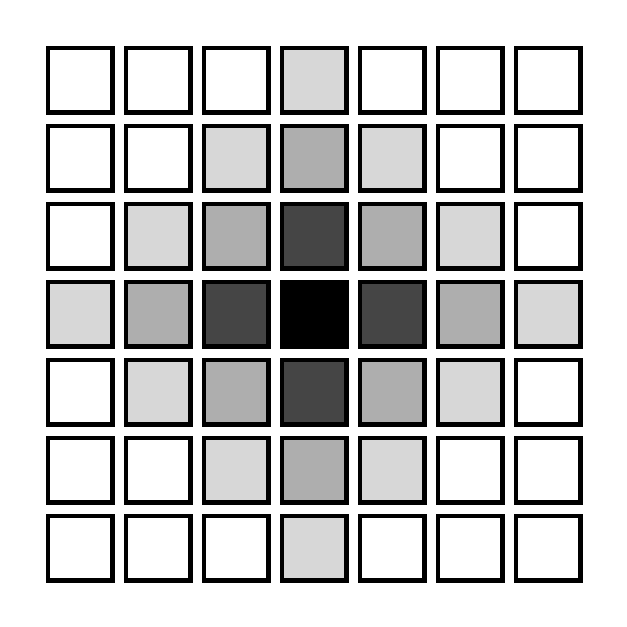
\includegraphics[width=0.4\textwidth]{vonneumanneighbor}}
%\subfigure{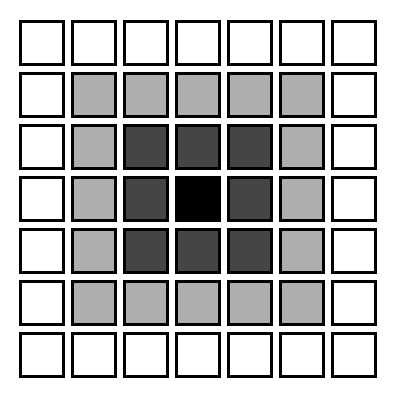
\includegraphics[width=0.4\textwidth]{mooreneighbor}}
%\caption{}
%\label{fig:masterslave}
%\end{figure}





%%%%%%%%%%%%%%%%%%%%%%%%%%%%%%%%%%%%%%%%%%%%%%%%%%%%%%%%%%%%%
\section{Population structure as a complex network}
\label{sec:structurecomplex}
%%%%%%%%%%%%%%%%%%%%%%%%%%%%%%%%%%%%%%%%%%%%%%%%%%%%%%%%%%%%%


To help understand the role of the population structure in a P2P EA, this section introduces the structural design of a simple and easy understandable complex network proposed by Watts and Strogatz in \cite{wattsstrogatz}. As described by the authors, the procedure for building a small-world topology can start from a ring lattice with $n$ vertices and $k$ edges per vertex. With a given probability $p$, each edge is rewired at random. Since the procedure does not allow duplicate edges, no edge is generated whenever it matches an existing one. This way for a rewiring factor of
$p=0$ the ring lattice is kept while for $p=1$ a random graph is generated. It has been shown that already for small values of $p$, the average distance between two nodes decreases rapidly. 


\begin{figure*}[htbp]
\centerline{\subfigure{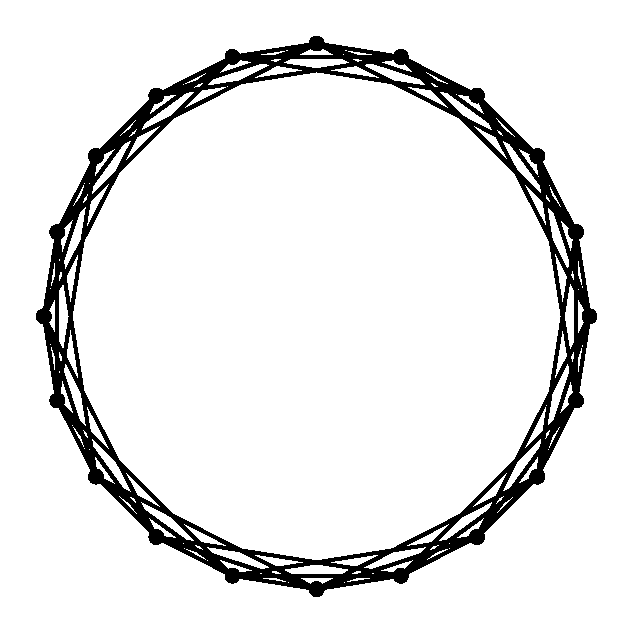
\includegraphics[width=1.5in]{WS-20-0000}
}
\hfil
\subfigure{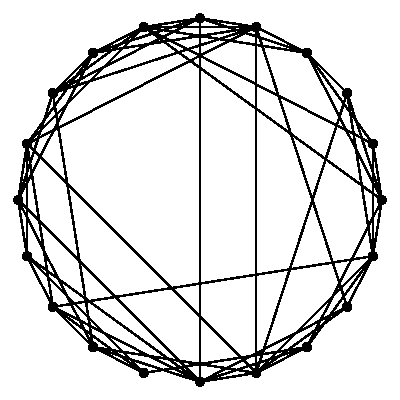
\includegraphics[width=1.5in]{WS-20-0200}
}
\hfil
\subfigure{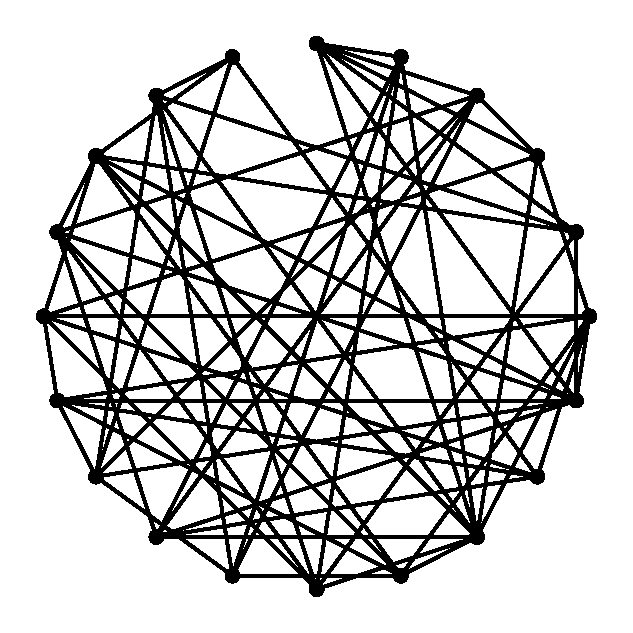
\includegraphics[width=1.5in]{WS-20-1000}
}}
\caption{Watts-Strogatz graphs with $n=20$ and $k=6$. From left to right, the original ring lattice for $p=0$, a small-world graph for $p=0.2$ and a random graph for $p=1$. 
}
\label{fig:small-world}
\end{figure*}


Figure \ref{fig:small-world} shows three stages of evolution of the Watts-Strogatz model in which the small-world graph preserves the high clustering coefficient of regular lattices and the small average path length of random graphs. Despite having a larger average path length than panmictic graphs, the inhomogeneity in such kind of topologies was shown by Giacobini et al. in \cite{giacobini:gecco05} to induce qualitatively similar selection pressures on EAs compared to panmictic population structures. 

The influence  in the environmental selection pressure of such population structures can be represented by their takeover time curves. Goldberg and Deb define in \cite{Goldberg91acomparative} the takeover time as the time that it takes for a single, best individual to take over the entire population with no mechanism other than selection. Hence, takeover time is the proportion of best individuals formulated as a function of time. 

\begin{figure*}[htbp]
\centerline{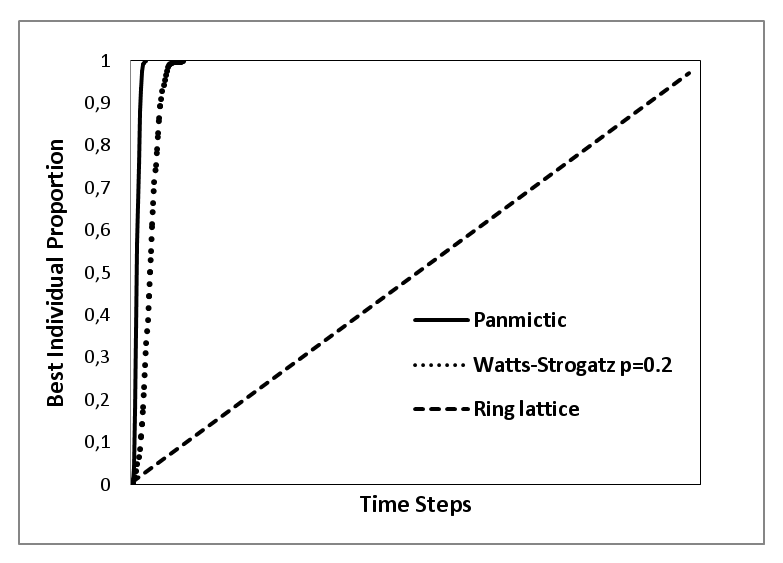
\includegraphics[width=0.7\textwidth]{takeoverwattsstrogatz}}
\caption{Takeover time curves in a panmictic population structure, Watts-Strogatz population structure with $p=0.2$ and the original ring lattice with $k=2$. All results averaged from 50 independent runs, for a population size of $n=1600$ and binary tournament. }
\label{fig:takeoversw}
\end{figure*}

Figure \ref{fig:takeoversw} shows that the takeover time curve in the Watts-Strogatz graph is similar to a panmictic graph meaning that the induced selection pressures using both topologies are roughly equivalent. As in Watts-Strogatz small-world topologies, this thesis will show that P2P topologies can induce similar selection pressures to the panmictic one, allowing in addition a better scalability behaviour at the lower edge cardinality of P2P systems.


%%%%%%%%%%%%%%%%%%%%%%%%%%%%%%%%%%%%%%%%%%%%%%%%%%%%%%%%%%%%%
\section{A review on Peer-to-Peer Evolutionary Algorithms}
\label{sec:p2peas}
%%%%%%%%%%%%%%%%%%%%%%%%%%%%%%%%%%%%%%%%%%%%%%%%%%%%%%%%%%%%%

A first insight from the sections above is that P2P EAs models should be closer to fine-grained approaches in order to be scalable. However, studying scalability in distributed EAs over P2P networks is not straightforward and is usually approached in two complementary ways, using real environments \cite{folino06:pcage} or using simulations \cite{balazs:evo09}; either way presents its own advantages and drawbacks.

% Este párrafo tampoco sé a santo de qué viene.
% "performing a real massively distributed and decentralised experiment" -> "experiments in real environments", así engancho con el párrafo anterior- Juanlu
On the one hand, experiments in real environments present some challenges that, so far, pose a whole set of practical problems beyond the state of the art. The main reason is the difficulty to
gather a large amount of reliable resources. Whenever the study
of scalability is reduced to a few peers, no conclusions about massive
scalability can be drawn. However, if the amount of peers is large
enough, other questions, such as fault tolerance, arise
\cite{merelo08:agajaj}.  
On the other hand, using simulations simplifies the analysis and allows focusing on the structural design since restrictions like the harnessing of computing power or the peers' failures disappear. The drawback in this case is that simulations imply a certain number of assumptions about the real environment; hence, they have to be well stated (e.g. representing a pessimistic scenario as in \cite{balazs:evo09}).



%Usa regarding lo menos que puedas, o 0.
In this context, some of the most relevant works that have tackled scalability using real enrironments are detailed bellow:
% NI itemize ni ná de ná?
% Itemizado - Juanlu


%%%%%%%%%%%%%%%%%%%
\begin{itemize}
\item {\em DREAM} \cite{arenas:dream}, is one of the pioneering frameworks for P2P EC, the proposal focuses on the distributed processing of EAs and uses the P2P engine DRM (Distributed Resource Machine) which is an implementation of the newscast protocol \cite{jelasity:newscast}. There are some other frameworks based on {\em DREAM} as {\em G2DGA} \cite{g2dga} which uses G2P2P instead of DRM and focuses on Genetic Algorithms among all the EAs paradigms.

\item Folino and Spezzano propose in \cite{folino06:pcage} the {\em P-CAGE} environment for EC in P2P
systems which is a hybrid model combining islands with cellular
EAs. Every peer holds an island and every island a cellular EA. Despite
results outperforming canonical EAs (either in execution time or
convergence speed), the scalability analysis is limited to ten peers and
the algorithm yields the best performance with five peers which points
to poor scalability. % Antes has usado runtime; usa siempre la misma
		     % palabra, o execution time o runtime. - JJ
		     % Execution time! - Juanlu

\item Lee proposes in \cite{lee:jade} a parallel system for EC using the P2P framework JADE. The optimisation is performed by three kinds of agents: state agents for controlling whether the peer is active or not, mobile agents for performing the evolutionary computation and the synchronising agent, a centralised agent for synchronising all the active peers. The algorithm's execution time speeds-up linearly but the scalability analysis is limited to eight nodes from which no conclusions about true scalability can be extracted. 
\end{itemize}
%%%%%%%%%%%%%%%%%%%

In addition to the previous approaches for real environments, some other works in the literature face the design of P2P EAs by means of simulations, focusing on the viability of the approaches rather than dealing with the harnessing of computing power.

%%%%%%%%%%%%%%%%%%%
\begin{itemize}

\item The self-organising topology evolutionary algorithm ({\em SOTEA}) by Whitacre et al. in \cite{sotea} is an EA designed for the sake of diversity maintenance. To this end, the authors focus on a self-organised population structure with the shape of a complex network. The network co-evolves with the EA by following two rules (from which a power law population structure emerges):
%%%%%%%%%%%%%%%%%%%%
\begin{enumerate}
\item Reproduction rule:
          When a new offspring is created, SOTEA adds a new node, this node is linked to its parent (asexual reproduction). The parent's connections are inherited by the offspring with certain probability $P_{add}$. In addition, all inherited connections are lost by the parent with probability $P_{remove}$.
\item Competition rule:
          A random selected individual competes with its less fit neighbour. From such a competition, the loser is killed and the winner inherits all its connections.
\end{enumerate}
%%%%%%%%%%%%%%%%%%%
By following these two rules, SOTEA keeps a better population diversity than the Cellular and Panmictic GA used as a baseline for comparison.
% todos estos sistemas son P2P, no distribuidos en general. Si cambias
% de sitio el capítulo siguiente quizás esté más justificado que te
% limites a esto. - JJ
% No entiendo muy bien esta apreciacion, tal vez porque en el momento de leerla los capitulos ya estan reestructurados y ahora no tenga sentido... no se :-( - Juanlu

\item Along the same lines of self-organised algorithms, Wickramasinghe et al. present in \cite{upali:adaptive}  a P2P EA with two particular properties: autonomous selection and natural reproduction. Autonomous selection means that the individuals in the population decide on their own whether and when they want to reproduce and to survive
without any central control. To this end, they use information on their own fitness
and estimations about the total population to support decision making. The second special feature, natural reproduction, means that birth and death decoupled
\cite{eiben2007}. That is, an individual can be removed without being replaced
by a child and a child can be born without removing an existing individual first.
This is highly uncommon in EAs and as a consequence, the population size varies
at run-time (just like in natural evolution) and a self-adjusting selection pressure
mechanism is needed to prevent population implosions or explosions.

\end{itemize}
%%%%%%%%%%%%%%%%%%%

Nevertheless and to the best of our knowledge, none of these approaches perform an integral analysis of viability taking into account the issues of decentralisation, scalability and fault-tolerance in P2P systems at once. Therefore, this thesis aims to present and analyse a simple and easy-understandable model for P2P EAs that cope with the mentioned issues, so that, the general viability of P2P EAs can be concluded.


%%%%%%%%%%%%%%%%%%%%%%%%%%%%%%%%%%%%%%%%%%%%%%%%%%%%%%%%%%%%%
\section{Summary}
\label{sec:peaconclusions}
%%%%%%%%%%%%%%%%%%%%%%%%%%%%%%%%%%%%%%%%%%%%%%%%%%%%%%%%%%%%%

This chapter describes the main parallel and distributed EA models reviewing the possible advantages and drawbacks of adapting a given model to a P2P system. To this aim, parallelism has been considered at two different levels in the structure of an EA, evaluation and population levels. The first takes adventage of the parallel evaluation of individuals on different processors in an approach known as global parallelisation. A global parallel EA keeps a single and centralised population that evolves following the same scheme than in the sequential mode. The centralised management of the evolutionary loop represents a bottleneck on the master node and linear speedups can be expected up to a few processors imposing, this way, a limitation to the massive scalability of P2P systems. In the second case, parallelism is considered at population level in which the global population is divided into several demes running on different processors and communicating with each other, that is, the algorithm is spatially structured. Spatially structured EAs can be classified in coarse-grained and fine-grained approaches depending on the parallelisation grain. In the coarse-grained approach, the population is divided in several panmictic subpopulations while in the fine-grained approach, individuals interact with each other by means of the population structure, so that, potentially, they can be placed on different processors. In a similar way that the global parallel EA, the spatially structured coarse-grained model has some difficulties to take advantage of a large number of resources, specially, when tackling large and difficult problems. However, fine-grained approaches seems to be more suitable for massive parallelisation and the population structure can be defined with the shape of a complex network as in the case of P2P systems.

Finally, some of the most relevant works in the literature of P2P EAs are presented showing the interest of the scientific community in this field of research. Nevertheless, we miss an integral analysis of viability  addressing  the issues of decentralisation, scalability and fault-tolerance. This thesis aims to tackle such issues in the following chapters.







%%%%%%%%%%%%%% Bibliografia %%%%%%%%%%%%%%%

%\bibliographystyle{alpha}  % Eliminarlo al compilar el documento maestro, ponerlo para compilarlo separado
%\bibliography{pea,p2pcomputing}% Eliminarlo al compilar el documento maestro, ponerlo para compilarlo separado

%\end{document}             % Eliminarlo al compilar el documento maestro, ponerlo para compilarlo separado
